\documentclass{article}
\usepackage[utf8]{inputenc}


\usepackage{float}
\usepackage{caption}



\usepackage{xcolor} 
\definecolor{myblue}{HTML}{ABDBE3}
\definecolor{myorange}{HTML}{FCAD68}


\usepackage{tikz}
\usetikzlibrary{shapes,arrows,fit,mindmap,positioning,arrows,matrix,calc} % TODO: only import want you really need

\tikzstyle{decision} = [diamond, draw, fill=myblue, 
text width=4.5em, text badly centered, node distance=2.5cm, inner sep=0pt]
\tikzstyle{block} = [rectangle, draw, 
fill=myorange, 
text width=5em, text centered, rounded corners, minimum height=4em]
\tikzstyle{line} = [draw, -latex']


\begin{document}

\begin{figure}[H]
\centering
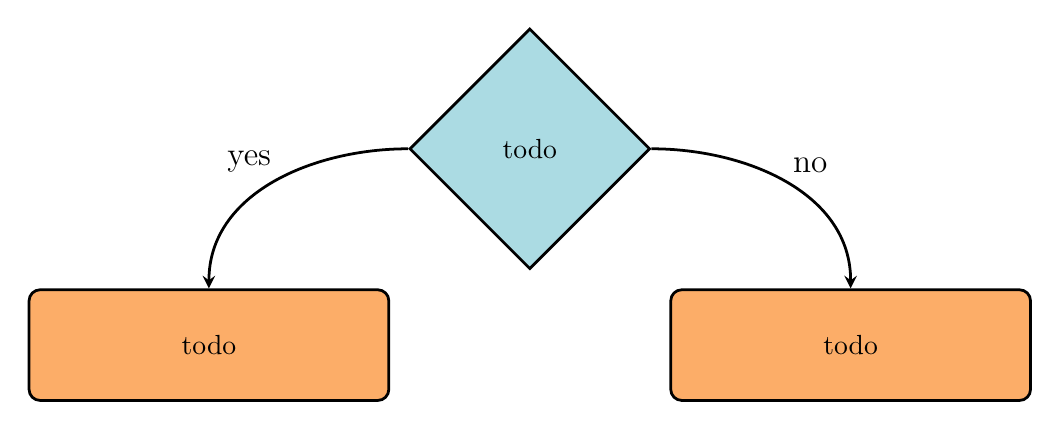
\begin{tikzpicture}]
    % Nodes
    \node [decision, text width=8em, line width=1pt] (first) {todo};

    \node [block, below left=1cm and 1cm of first, minimum width=13em, text width=12em, line width=1pt] (path_exists) {todo};
    \node [block, below right=1cm and 1cm of first, minimum width=13em, text width=12em, line width=1pt] (path_does_not_exists) {todo};

    \draw[>=stealth, ->, line width=1.0pt] (first.west) [out=180, in=90] to node[xshift=-0.3cm, above] {\large yes} (path_exists.north);
    \draw[>=stealth, ->, line width=1.0pt] (first.east) [out=0, in=90] to node[xshift=0.3cm, above] {\large no} (path_does_not_exists.north);

\end{tikzpicture}
\caption*{todo}%
\end{figure}

\end{document}
